\documentclass{article}

\usepackage[norsk]{babel}
\usepackage[margin=1.5in]{geometry}
\usepackage{graphicx}
\usepackage{wrapfig}

\usepackage{caption}
\usepackage{subcaption}

\usepackage{array}
\usepackage{multirow}
\usepackage{diagbox}
\usepackage{hyperref}

\usepackage{listings}
\usepackage{color}
\usepackage{xcolor}

\definecolor{light-gray}{gray}{0.95}
\newcommand{\code}[1]{\colorbox{light-gray}{\texttt{#1}}}

\newlength{\bcw}
\setlength{\bcw}{2.5em}

\title{IDATT2104 - Datakom Oblig 2}
\author{Jakob Grønhaug (jakobkg@stud.ntnu.no)}

\begin{document}
\maketitle

\tableofcontents

\section{Websocket}
\subsection{Teori}

\subsubsection{Forskjeller mellom HTTP og Websocket}

Det er flere likheter og forskjeller mellom HTTP og Websocket. For begynner alle Websocket-forbindelser med et handshake over HTTP, så man kan ikke implementere Websocket uten å først ha implementert ihvertfall noen deler av HTTP.

Den viktigste forskjellen er at HTTP er bygd på en rigid struktur der hver interaksjon følger formatet \code{klient sender forespørsel\rightarrow tjener sender svar}. I HTTP er det et 1:1-forhold mellom forespørsler fra klienten og svar fra tjeneren, og det er alltid klienten som tar initiativ til en slik interaksjon. Dette har visse begrensninger, la oss for eksempel si en klient venter på at tjeneren skal bli ferdig med en større databehandlingsjobb, eller venter på en tilstandsendring av noen form. 

Siden HTTP ikke tillater at tjeneren tar initiativ til sending av data til en klient må klienten selv spørre tjeneren med jevne mellomrom 'er du ferdig enda? er du ferdig enda? er du ferdig enda?'. Dette kan føre til at klienten må generere mange unødvendige forespørsler, og tjeneren må bruke tid og ressurser på å svare 'Nei jeg er ikke ferdig enda' i stedet for å kunne vie disse ressursene til å utføre jobben klienten venter på. Websocket har ikke denne samme strukturen med 'forespørsel\rightarrow respons' og kan dermed unngå den samme problemstillingen. Etter at handshake er gjennomført kan tjeneren sende klienten varsling om at ny data/tilstand er tilgjengelig uten at klienten trenger å spørre gjentatte ganger!

\subsubsection{Sikkerhetsmekanisme i Websocket}

Websocket er i seg selv ikke en sikkerhetsorientert protokoll. Enkelte meldinger er maskerte, men masken som brukes for å demaskere meldingene sendes i headeren til de samme meldingene, så dette må ikke forveksles med faktisk kryptering. Websocket bruker \texttt{Origin}-headeren ved oppkobling på samme måte som HTTP for å gi tjenere muligheten til å avvise koblinger fra ukjente klienter, men dette er kun nyttig for koblinger som opprettes gjennom nettlesere. Andre klienter kan sende hva de vil i dette header-feltet, så det burde ikke regnes som en faktisk sikkerhet.

En sikrest mulig Websocket-kobling oppnås ved å initiere den over HTTPS heller enn HTTP, i dette tilfellet vil Websocket-koblingen arve TLS-koblingen fra HTTPS og holde trafikken kryptert.

\subsection{Dokumentasjon}
\subsubsection{Oppkobling/handshake}

Ifølge Websocket-standarden (\href{https://www.rfc-editor.org/rfc/rfc6455.html}{RFC 6455}) er en Websocket-kobling noe en HTTP-klient og HTTP-tjener blir enige om å opprette. Først sender klienten en GET-forespørsel, og inkluderer feltet \code{Upgrade: websocket} i headeren til forespørselen. Denne forespørselen skal også spesifisere hvilken versjon av Websocket som skal brukes, og inneholde en tilfeldig nøkkel\footnote{Denne tilfeldige nøkkelen, og senere maskering av meldinger fra klienter til tjenere, brukes for å unngå at proxyer og cache som kan ligge mellom klienten og tjeneren svarer 'på vegne av' tjeneren med en forhåndslagret kopi av en tidligere respons. Ved bruk av et tilfeldig element som nøkkelen i handshake og maskering av meldinger sørger man for at den faktiske dataen som sendes over nettverket er forskjellig hver gang selv om meldingen som ble sendt kanskje er den samme.} \code{Sec-Websocket-Key} på 16 byte, kodet i Base64, som tjeneren skal bruke for å verifisere svaret sitt.

Tjeneren skal så svare med en HTTP-respons med status \code{101 Switching Protocols} som må inneholde header-feltene \code{Upgrade: websocket} og \code{Connection: upgrade}, og et header-felt \code{Sec-Websocket-Accept}. Dette feltet er spesielt, og verdien som skal puttes her må utledes fra den tilfeldige nøkkelen som klienten sendte i sin del av handshaket. Tjeneren skal ta denne nøkkelen og legge til \code{258EAFA5-E914-47DA-95CA-C5AB0DC85B11} på slutten av den. Denne teksten er alltid den samme, og er oppgitt i spesifikasjonen. Om klienten sender nøkkelen \code{iMTLEqLRkU4JmXSI36YK8g==} skal tjeneren altså ende opp med \code{iMTLEqLRkU4JmXSI36YK8g==258EAFA5-E914-47DA-95CA-C5AB0DC85B11}. Videre skal tjeneren bruke SHA1-algoritmen til å beregne hashen til denne teksten. En SHA1-hash er alltid 20 bytes lang, og hashen av eksempel-nøkkelen blir

\begin{center}
    \code{0xEB, 0xE8, 0xD4, 0xEA, 0x62, 0xC6, 0x38, 0x47, 0x56, 0x12,}
    
    \code{0xB9, 0xD3, 0x48, 0x58, 0x38, 0xE7, 0x76, 0x0E, 0x77, 0x19 }
\end{center}

\begin{figure}[ht]
    \centering
    \begin{subfigure}{\linewidth}
        \centering
        \includegraphics*[width=\linewidth]{illustrasjoner/WS_handshake.png}
        \caption{Websocket-handshake slik det fremstår i pakkelisten i Wireshark}
    \end{subfigure}

    \begin{subfigure}{.48\linewidth}
        \centering
        \includegraphics*[width=\linewidth]{illustrasjoner/WS_handshake_klient.png}
        \caption{Klientens del av handshake}
    \end{subfigure}
    \hfill
    \begin{subfigure}{.48\linewidth}
        \centering
        \includegraphics*[width=\linewidth]{illustrasjoner/WS_handshake_tjener.png}
        \caption{Tjenerens del av handshake}
    \end{subfigure}
    \caption{Skjermbilder av Websocket-handshaket i Wireshark}
    \label{fig:ws_handshake}
\end{figure}

Tjeneren må så kode denne hashen som Base64, og denne Base64-strengen er det som skal sendes fra tjeneren i \code{Sec-Websocket-Accept}-feltet i headeren. I dette spesifikke eksempelet blir dette feltet \code{Sec-Websocket-Accept: 6+jU6mLGOEdWErnTSFg453YOdxk=}. Skjermbildene i figur \ref{fig:ws_handshake} viser dette eksempel-handshaket i faktisk trafikk.

\subsubsection{Meldinger fra klient til tjener}

Når oppkoblingen er utført som beskrevet over er Websocket-forbindelsen opprettet og klar for trafikk! Både klient og tjener kan sende data over denne koblingen når de vil, med hovedforskjell at klienter alltid skal sende meldingene sine med maskering, mens en tjener ikke trenger å gjøre det.

Denne maskeringen er ment å hindre problemer som kan oppstå dersom en hjelpsom proxy eller cache mellom klienten og tjeneren svarer på vegne av tjeneren i et forsøk på å korte ned svartiden. I mange tilfeller er dette ønskelig på internett, dersom en klient sender en forespørsel om samme bilde to ganger med kort mellomrom er det ikke urimelig å anta at bildet er det samme ved andre forespørsel som ved første, og dermed kan en proxy sende en mellomlagret kopi av bildet i stedet for å sende forespørselen helt til tjeneren.
Ved websocket-trafikk er det ikke gitt at samme forespørsel burde ha samme svar, la oss for eksempel se for oss et enkelt database-aktig system med en websocket-klient. En interaksjon med denne databasen kan se slik ut:

\begin{quote}
\tt
    1) Klient: USE TABLE butikker; \\
    2) Tjener: OK \\
    3) Klient: SELECT *; \\
    4) Tjener: \{JSON-data om butikker\} \\
    5) Klient: USE TABLE ansatte; \\
    6) Tjener: OK \\
    7) Klient: SELECT *; \\
    8) Tjener: \{JSON-data om ansatte\} \\
\end{quote}

Dersom denne interaksjonen gikk via en slik hjelpsom proxy kunne denne ha mellomlagret responsen med butikk-data i linjer 3-4, slik at når klienten spør om ansatt-data i linje 7 kommer svaret med butikk-data igjen fra proxyen siden forespørselen som er identisk. Ikke bra! For å unngå at dette skal kunne skje må det tilføres et element av tilfeldighet slik at de to forespørslene på linje 3 og linje 6 ser forskjellige ut for mellomstopp på nettverket selv om den faktiske meldingen er den samme. Dette løser Websocket-spesifikasjonen ved å kreve at alle meldinger fra en klient er maskert med en tilfeldig generert maske, mer om dette senere.

Meldinger over Websocket sendes i form av ett eller flere fragment, hvor alle fragmenter følger en bestemt struktur. I denne oppgaven var det kun krav om å implementere meldinger på ett fragment med meldingslengde på opp til 125 bytes. Slike fragmenter har struktur som vist i figur \ref{fig:fragmentstruktur}.

\begin{figure}[ht]
    \centering
    \begin{tabular}[h]{|c|w{c}{\bcw}|w{c}{\bcw}|w{c}{\bcw}|w{c}{\bcw}|w{c}{\bcw}|w{c}{\bcw}|w{c}{\bcw}|w{c}{\bcw}|}
        \hline
        \diagbox[width=4em]{Byte}{Bit} & 0 & 1 & 2 & 3 & 4 & 5 & 6 & 7 \\
        \hline
        1 & \tt{FIN} & \multicolumn{3}{c|}{\tt{RESERVERT}} & \multicolumn{4}{c|}{\tt{MELDINGSTYPE}} \\
        \hline
        2 & \tt{MASK} & \multicolumn{7}{c|}{\tt{MELDINGSLENGDE}} \\
        \hline
        3 & \multicolumn{8}{c|}{\multirow{4}{*}{\tt{MASKERINGSNØKKEL}}} \\
        4 & \multicolumn{8}{c|}{\multirow{4}{*}{}} \\
        5 & \multicolumn{8}{c|}{\multirow{4}{*}{}} \\
        6 & \multicolumn{8}{c|}{\multirow{4}{*}{}} \\
        \hline 
        ... & \multicolumn{8}{c|}{\tt{MELDINGSDATA}} \\
        \hline
    \end{tabular}
    \caption{Strukturen til et Websocket-fragment fra en klient til en tjener, forenklet fra \href{https://www.rfc-editor.org/rfc/rfc6455\#section-5.2}{RFC 6455, 5.2}}
    \label{fig:fragmentstruktur}
\end{figure}

I første byte av et fragment har vi en bit markert \code{FIN} som indikerer hvorvidt dette fragmentet er det siste i en melding. Siden det kun skal støttes korte meldinger antar jeg i implementasjonen min at \code{FIN}-biten alltid er satt til \texttt{1}. De neste tre bitene er reserverte for utvidelser av Websocket-spesifikasjonen. Siden tjeneren min ikke er ment å støtte noen slike utvidelser antar jeg at disse tre bitene har verdi \texttt{0}. De siste fire bits angir meldingstypen, og kan ha et par forskjellige verdier. Siden jeg kun ønsker å støtte tekst-meldinger kan jeg anta at disse fire bits har verdi \code{0b0001}. Totalt kan jeg altså alltid anta at første byte har verdi \code{0b10000001}/\code{0x81}.

Andre byte av fragmentet starter med \code{MASK}-biten som forteller oss hvorvidt dataen i fragmentet er maskert eller ikke. Websocket-spesifikasjonen angir at alle meldinger som sendes fra en klient til en tjener skal være maskert, så tjeneren jeg har implementert antar at \code{MASK}-biten alltid er \texttt{1}. De andre syv bitene i denne byten angir meldingslengden. I en fullstendig implementasjon av Websocket-standarden kan denne lengden være angitt her i syv bits eller i de neste to eller åtte bytes. Den faktiske standarden sier at om disse syv bits har verdier \code{0b1111110} er den faktiske størrelsen angitt i de neste to bytes, og om de syv bitene er \code{0b1111111} er den faktiske størrelsen angitt i de påfølgende åtte bytes. Siden jeg bare vil støtte korte meldinger antar jeg at lengden er mellom \code{0b0000001} (1) og \code{0b1111101} (125) slik at headeren alltid har samme størrelse og layout. Dersom større meldinger skulle vært implementert ville det vært tre forskjellige layouts og størrelser headeren kunne hatt basert på om meldingslengden får plass i syv bits, to byte eller åtte byte.

De neste fire bytes i fragmentet er en tilfeldig generert maskeringsnøkkel. Dataen som sendes fra en klient er maskert med denne masken, og den samme masken kan dermed brukes til å demaskere dataen igjen etter at den er mottatt. Maskeringsnøkkelen er tilfeldig generert av klienten og skal være forskjellig for hvert fragment, i motsetning til nøklene som brukes i kryptert kommunikasjon som f.eks. TLS der et par 'session keys' genereres ved oppkobling og gjenbrukes gjennom en hel sesjon.

La oss se på et helt fragment, der en klient sender teksten \code{hallo} til en tjener. Første byte vet vi allerede at skal være \code{0x81} for å indikere at dette er en tekstmelding og dette fragmentet inneholder hele meldingen. Andre byte skal indikere at meldingen er maskert og har en lengde på fem bytes for de fem bokstavene, så denne blir \code{0b10000101}/\code{0x85}. Neste fire bytes skal være tilfeldig valgte, så jeg triller noen terninger og ender opp med maskeringsnøkkelen \code{0x1D, 0x43, 0x9F, 0xBF}. Meldingen \code{hallo} kan kodes til fem bytes \code{0x68, 0x61, 0x6c, 0x6c, 0x6f}. For å maskere dataen før sending tar vi første byte av dataen XOR første byte av masken, andre byte av dataen XOR andre byte av masken, osv. Når det er flere bytes i meldingen enn i nøkkelen rykker vi tilbake til starten av nøkkelen når vi når slutten av den, slik at femte byte av dataen maskeres med første byte av nøkkelen. Den maskerte dataen blir dermed 

\begin{center}
    \begin{tabular*}{.492\linewidth}[H]{cccccc}
        & \tt0x68 & \tt0x61 & \tt0x6C & \tt0x6C & \tt0x6F \\
        \tt XOR & \tt0x1D & \tt0x43 & \tt0x9F & \tt0xBF & \tt0x1D \\
        \hline
        \tt = & \tt0x75 & \tt0x22 & \tt0xF3 & \tt0xD3 & \tt0x72 \\
        \hline
    \end{tabular*}
\end{center}

Med det har vi hele fragmentet klart! Dataen som sendes fra klienten til tjeneren over nettverket er til sammen 

\begin{center}
    \code{0x81, 0x85, 0x1D, 0x43, 0x9F, 0xBF, 0x75, 0x22, 0xF3, 0xD3, 0x72}
\end{center}

\subsubsection{Meldinger fra tjener til klient}

Meldinger fra tjenere til klienter er heldigvis mye greiere. All makseringen vi har måttet drive med så langt er kun for å unngå problematikk som kan oppstå dersom en hjelpsom proxy mellomlagrer et svar fra tjeneren. Denne problematikken finnes ikke den andre veien, og dermed trenger ikke meldingene fra en tjener til en klient å maskeres på samme måte.

\begin{figure}[ht]
    \centering
    \begin{tabular}[h]{|c|w{c}{\bcw}|w{c}{\bcw}|w{c}{\bcw}|w{c}{\bcw}|w{c}{\bcw}|w{c}{\bcw}|w{c}{\bcw}|w{c}{\bcw}|}
        \hline
        \diagbox[width=4em]{Byte}{Bit} & 0 & 1 & 2 & 3 & 4 & 5 & 6 & 7 \\
        \hline
        1 & \tt{FIN} & \multicolumn{3}{c|}{\tt{RESERVERT}} & \multicolumn{4}{c|}{\tt{MELDINGSTYPE}} \\
        \hline
        2 & \tt{MASK} & \multicolumn{7}{c|}{\tt{MELDINGSLENGDE}} \\
        \hline 
        ... & \multicolumn{8}{c|}{\tt{MELDINGSDATA}} \\
        \hline
    \end{tabular}
    \caption{Strukturen til et Websocket-fragment fra en tjener til en klient, forenklet fra \href{https://www.rfc-editor.org/rfc/rfc6455\#section-5.2}{RFC 6455, 5.2}}
    \label{fig:fragmentstruktur_tjener}
\end{figure}

Akkurat som for klienter må også tjeneren sette opp første byte med en bit som markerer at dette fragmentet er det siste i meldingen sin, tre reserverte bits og fire bits som markerer meldingstype. For korte meldinger med tekst-innhold vil denne alltid være \code{0b10000001} eller \code{0x81}, akkurat som vi så tidligere.

Andre byte inneholder maske-biten, som alltid vil være 0 siden meldinger fra tjenere ikke trenger maskeres. Som tidligere inneholder de neste syv bits meldingslengden, gitt at meldingen ikke er lengre enn 125 bytes lang. Om en tjener sender meldingen \code{hallo} til en klient vil lengden være 5, så denne byten blir \code{0b00000101} eller \code{0x05}.

Det er alt av headere! Ingen maskeringsnøkkel eller andre finurlige saker. Dersom en tjener skal sende melding med teksten \code{hallo} til en klient vil meldingsdataen kun være teksten uten noen ekstra koding. Som vi så tidligere er denne teksten representert som bytes som \code{0x68, 0x61, 0x6c, 0x6c, 0x6f}. Disse bytene setter vi rett inn i meldingen, så den totale meldingen blir:

\begin{center}
    \code{0x81, 0x05, 0x68, 0x61, 0x6c, 0x6c, 0x6f}
\end{center}

De to meldingene der klient og tjener sier \code{hallo} ser som forventet ut i Wireshark:

\begin{figure}[h]
    \centering
    \begin{subfigure}{.48\linewidth}
        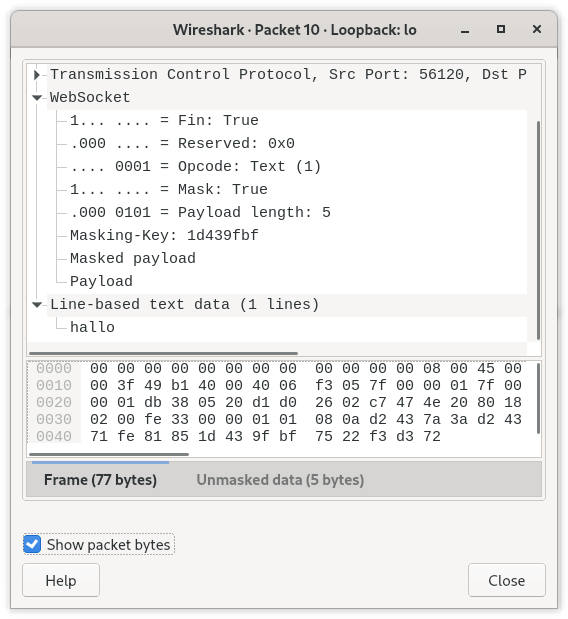
\includegraphics[width=\linewidth]{illustrasjoner/WS_fra_klient.png}
    \end{subfigure}
    \hfill
    \begin{subfigure}{.48\linewidth}
        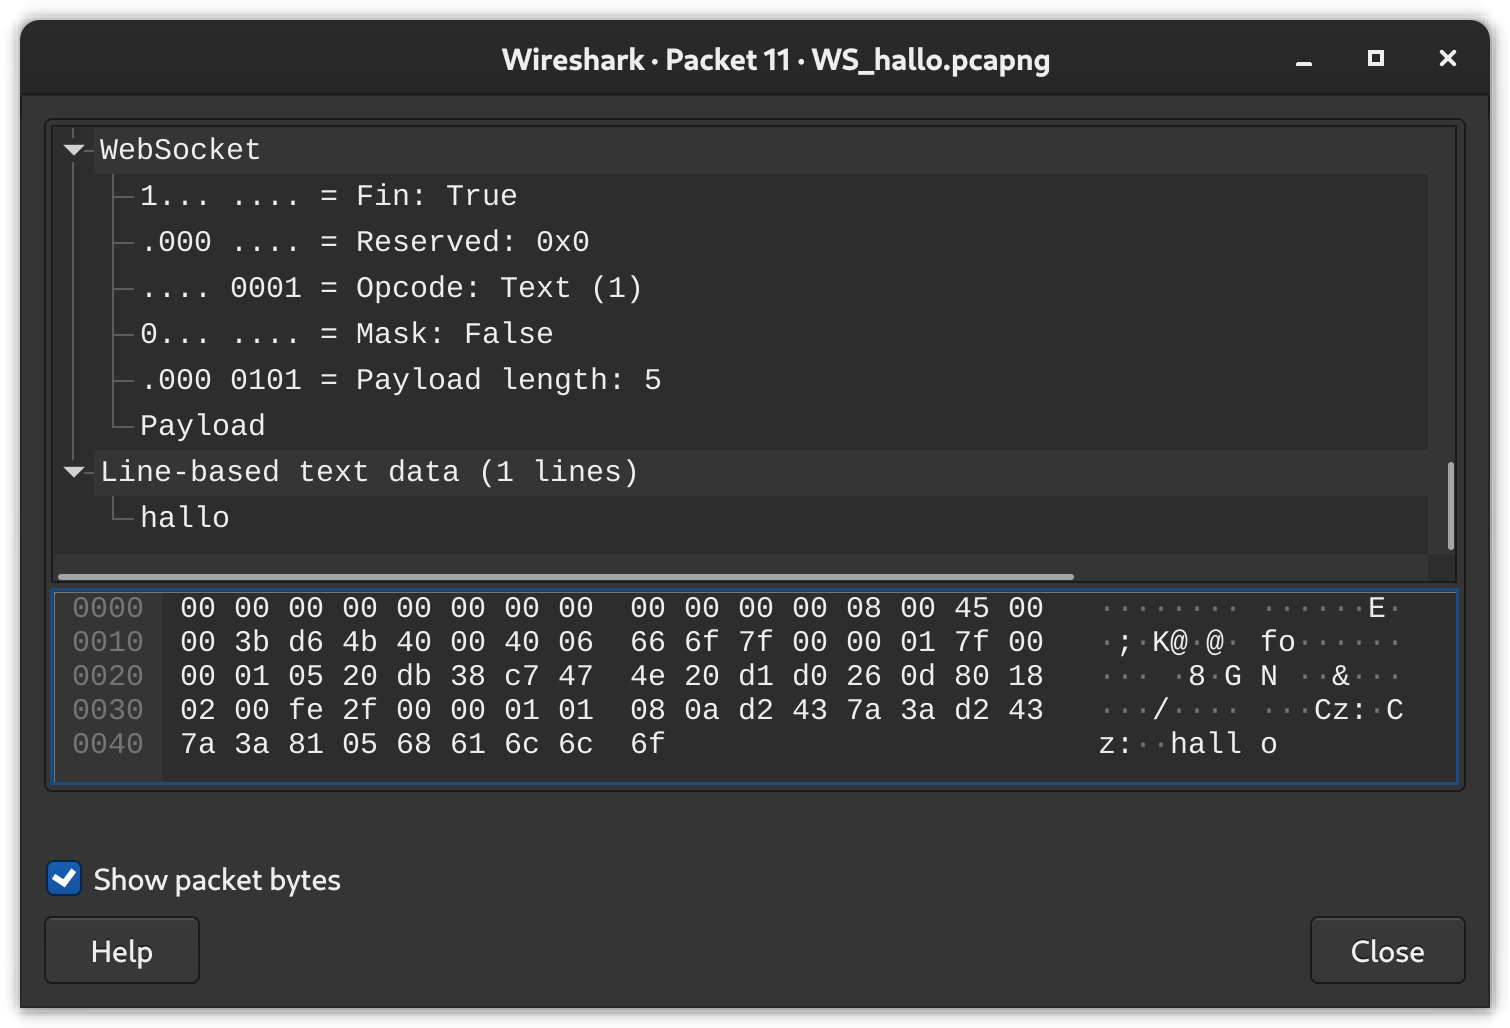
\includegraphics[width=\linewidth]{illustrasjoner/WS_fra_tjener.png}
    \end{subfigure}
\end{figure}

\section{SSH}

\subsection{Etablering av sikker forbindelse}

SSH bruker TCP på transportlaget, etter at TCP-handshake er utført og oppkobling er gjort har SSH sitt eget handshake. Klient og tjener kommuniserer først hvilke versjoner av SSH de støtter, og deretter hvilke krypteringsalgoritmer de tilbyr for å velge sterkest mulig kryptering. Klienten og tjeneren oppretter så hvert sitt nøkkelpar med offentlige og private nøkler, og utveksler offentlige nøkler. Nå som klienten og tjeneren har hverandres offentlige nøkler kan klienten kryptere kommunikasjon med tjenerens offentlige nøkkel, og dermed sikre at kun tjeneren kan dekryptere kommunikasjonen ved å bruke sin private nøkkel (og omvendt). Denne utvekslingen av nøkler kan sees i pakkefangsten i Wireshark i figur \ref*{fig:SSH_nøkler}

\begin{figure}[h]
    \centering
    \includegraphics[width=\linewidth]{illustrasjoner/SSH_nøkkelbytte.png}
    \caption{Handshake og nøkkelutveksling mellom klient og tjener med SSH}
    \label{fig:SSH_nøkler}
\end{figure}

\subsection{Autentisering av brukeren}

Nå som klienten og tjeneren har etablert en sikker kobling er neste steg at brukeren må bekrefte at de faktisk skal ha tilgang til tjeneren de prøver å koble seg til. Dette foregår stort sett på to måter, enten ved passord-autentisering eller ved nøkkel-autentisering.

Ved passord-autentisering spør tjeneren enkelt og greit om passordet til brukerkontoen, som brukeren skriver inn og sender tilbake for å autentisere seg og starte sesjonen sin. Det er vanskelig å hindre en ondsinnet aktør fra å spamme en tjener med påloggingsforsøk med forskjellige passord, så dette anses som en sårbar autentiseringsform og anbefales generelt ikke.

Nøkkel-autentisering fungerer ved at brukeren genererer et nøkkelpar med en privat og en offentlig nøkkel, og på forhånd registrerer sin offentlige nøkkel på tjeneren de ønsker å logge inn på. Når brukeren logger på tjeneren med SSH med nøkkel-autentisering genererer tjeneren et tilfeldig tall, krypterer det med brukerens offentlige nøkkel og sender det til brukerens klient. Dersom brukeren er den de utgir seg for å være vil de fint kunne dekryptere dette tilfeldige tallet med sin private nøkkel for så å generere en hash av dette og sende tilbake til tjeneren. Så lenge klienten og tjeneren kommer frem til samme hash kan tjeneren stole på at brukeren er den de utgir seg for å være, og slippes inn.

All denne trafikken er kryptert og vil ikke kunne sees i Wireshark.

\end{document}